\section{Films and disorder}\label{sec:15.3}

An electron in a clean aluminum crystal crosses a Cooper pair, \SI{2.4}{\micro m} across (\cref{sec:7.2}), without scattering, and the loss functions of \cref{sec:15.1,sec:15.2} assume exactly that. The sensors that count broken pairs, however, are films. In a \SI{50}{nm} aluminum film an electron reaches a surface after at most about \SI{50}{nm}. In the amorphous tungsten silicide of the QROCODILE dark-matter search, whose sensors are superconducting microwires patterned from a layer \SI{2}{nm} thick~\cite{baudis2025first}, it scatters after a few tenths of a nanometer, about once per interatomic distance. At the momentum transfers of keV-mass dark matter these collisions raise the normal-state loss function of the aluminum film about twentyfold. They also change the loss function at the pair-breaking edge, and a film thinner than $1/q$ screens like a sheet rather than like a bulk metal.

\subsection{Mean free path and Anderson's theorem}\label{sec:15.3-dirty}

The rate $\gamma_{\mathrm{rel}}$ at which collisions relax the momentum of an electron (\cref{sec:4.5}) sets two lengths. An electron at the Fermi surface travels the \emph{mean free path}
\begin{equation}
  \mathfrak{l}_e = \frac{v_{\mathrm{F}}}{\gamma_{\mathrm{rel}}}, \qquad D_{\mathrm{diff}} = \frac{v_{\mathrm{F}}\mathfrak{l}_e}{3} ,
  \label{eq:15.3-le}
\end{equation}
between collisions, and over many collisions it performs a random walk with diffusion constant $D_{\mathrm{diff}}$. The second relation follows from free flights of exponentially distributed length, which have $\langle s^2\rangle = 2\mathfrak{l}_e^2$, one per time $1/\gamma_{\mathrm{rel}}$ in a random direction, so that $\langle r^2\rangle = 2\mathfrak{l}_e^2\gamma_{\mathrm{rel}}t = 6D_{\mathrm{diff}}t$. The dc resistivity measures $\mathfrak{l}_e$. The Drude conductivity of \cref{sec:4.5} is $\nd_ee^2/(m_e\gamma_{\mathrm{rel}})$ in SI units, and with $\nd_e = k_{\mathrm{F}}^3/3\pi^2$ and $v_{\mathrm{F}} = \hbar k_{\mathrm{F}}/m_e$ the resistivity $\rho_{\mathrm{el}}$ obeys
\begin{equation}
  \rho_{\mathrm{el}}\,\mathfrak{l}_e = \frac{3\pi^2\hbar}{e^2k_{\mathrm{F}}^2} ,
  \label{eq:15.3-rho}
\end{equation}
a constant of the metal. For the free-electron gas of aluminum (\cref{sec:15.1-rate}) it is \SI{3.98e-16}{\ohm.m^2}, and a film with $\mathfrak{l}_e = \SI{50}{nm}$ has a residual resistivity of \SI{0.80}{\micro\ohm.cm} and $\gamma_{\mathrm{rel}} = \SI{26.7}{meV}$. We take $\mathfrak{l}_e$ equal to the thickness, $d_{\mathrm{film}} = \SI{50}{nm}$, as for a film whose surfaces scatter electrons diffusely; a measured residual resistivity replaces this choice through \cref{eq:15.3-rho}.

Which theory applies depends on three ratios: $q\mathfrak{l}_e$, $\mathfrak{l}_e/\xi_{\mathrm{coh}}$ and $k_{\mathrm{F}}\mathfrak{l}_e$. The first, $q\mathfrak{l}_e$, is the distance between collisions in units of the length $1/q$ of the perturbation. For $q\mathfrak{l}_e \gg 1$ the electrons are \emph{ballistic} on the scale $1/q$, and the response is that of the clean gas; for $q\mathfrak{l}_e \ll 1$ they are \emph{diffusive}, and a density disturbance spreads by diffusion. The second compares $\mathfrak{l}_e$ with the coherence length $\xi_{\mathrm{coh}} = v_{\mathrm{F}}/\pi\Delta_{\mathrm{BCS}}$, the size of a pair (\cref{sec:7.2}). A superconductor with $\mathfrak{l}_e \gg \xi_{\mathrm{coh}}$ is \emph{clean}, and one with $\mathfrak{l}_e \ll \xi_{\mathrm{coh}}$ is in the \emph{dirty limit}: each pair is spread over many impurities. For aluminum $\xi_{\mathrm{coh}} = \SI{2.4}{\micro m}$ with the free-electron $v_{\mathrm{F}}$, and the coherence length tabulated for aluminum is \SI{1.6}{\micro m}~\cite[Ch.~10, Table~5]{kittel2005introduction}; the clean results of \cref{sec:15.1,sec:15.2} need a mean free path long compared with either, which only bulk high-purity crystals have. The third ratio, $k_{\mathrm{F}}\mathfrak{l}_e$, is the mean free path in units of the electron wavelength. Disorder is weak for $k_{\mathrm{F}}\mathfrak{l}_e \gg 1$, where an electron still has a well-defined momentum between collisions, and strong near the Ioffe--Regel limit $k_{\mathrm{F}}\mathfrak{l}_e \approx 1$, where it does not. \Cref{tab:15-disorder} lists the three numbers for the aluminum film and for amorphous WSi. The aluminum film is weakly disordered, dirty, and diffusive at the momenta that keV-mass dark matter transfers; WSi is strongly disordered.

\begin{table}[tbp]
  \centering
  \caption{Disorder parameters of two superconducting sensor materials. Aluminum film: free-electron gas with $k_{\mathrm{F}} = \SI{1.75}{\angstrom^{-1}}$ and $v_{\mathrm{F}} = \num{6.75e-3}$, mean free path taken equal to the thickness of \SI{50}{nm}, coherence length $v_{\mathrm{F}}/\pi\Delta_{\mathrm{BCS}}$ with the bulk gap \SI{0.18}{meV}. Amorphous W$_x$Si$_{1-x}$: \SI{5}{nm} films with $x = 0.75$--0.85~\cite[Table~I]{zhang2016characteristics}; the range of $\mathfrak{l}_e$ comes from combining the measured diffusion constant (lower end) or the measured resistivity (upper end) with the free-electron gas at $E_{\mathrm{F}} = \SI{7}{eV}$; the coherence length is the measured Ginzburg--Landau value. The pair-breaking edge is $q = 2\Delta_{\mathrm{BCS}}/v_{\mathrm{max}}$, the smallest momentum transfer at which a halo particle can deposit $2\Delta_{\mathrm{BCS}}$; WSi has $\Delta_{\mathrm{BCS}} = \SI{0.263}{meV}$.}
  \label{tab:15-disorder}
  \begin{tabular}{@{}lcc@{}}
    \toprule
    & Al film, \SI{50}{nm} & amorphous WSi \\
    \midrule
    mean free path $\mathfrak{l}_e$ & \SI{50}{nm} & 0.13--\SI{0.41}{nm} \\
    relaxation rate $\gamma_{\mathrm{rel}}$ & \SI{27}{meV} & 2.5--\SI{7.7}{eV} \\
    $k_{\mathrm{F}}\mathfrak{l}_e$ & 874 & 1.8--5.5 \\
    $\mathfrak{l}_e/\xi_{\mathrm{coh}}$ & 0.021 & 0.02--0.06 \\
    $q\mathfrak{l}_e$ at the pair-breaking edge & 0.034 & (1.4--4.1)$\times10^{-4}$ \\
    $q\mathfrak{l}_e$ at $q = \SI{1}{keV}$ & 253 & 0.7--2.1 \\
    \bottomrule
  \end{tabular}
\end{table}

In the dirty limit the plane waves of \cref{sec:7.2} are no longer eigenstates, and the BCS construction has to be redone. Anderson~\cite{anderson1959theory} noticed that nonmagnetic impurities do not break time reversal. Every exact one-electron eigenstate $\psi_n$ of the disordered metal has a time-reversed partner $\psi_n^*$ at the same energy. He paired $\psi_n$ with $\psi_n^*$, in place of $\vect{k}$ with $-\vect{k}$, and took the attraction constant between the exact states within $\omega_{\mathrm{D}}$ of the Fermi level. The reduced Hamiltonian of \cref{eq:7.2-HBCS} then leads to the gap equation of \cref{eq:7.2-gap} with the density of states of the exact states at the Fermi level in place of $\mathcal{N}_{\mathrm{F}}$. Weak disorder changes that density of states only at relative order $1/k_{\mathrm{F}}\mathfrak{l}_e$, and nonmagnetic disorder leaves $\Delta_{\mathrm{BCS}}$ and $T_c$ at their clean values. This is \emph{Anderson's theorem}. Magnetic impurities break time reversal, the partner states no longer pair, and the gap falls. For a weakly disordered film the pair-breaking threshold is still $2\Delta_{\mathrm{BCS}}$, with the gap of the film, measured through its $T_c$ or by tunneling (\cref{sec:15.1-al}). The response, on the other hand, does change with disorder, because the matrix elements of $\ee^{\ii\vect{q}\cdot\vect{r}}$ between exact states are not those between plane waves.

\subsection{Relaxation-time loss functions}\label{sec:15.3-mermin}

Collisions enter the loss function through the Mermin dielectric function of \cref{eq:4.5-mermin}, which relaxes the electrons toward local equilibrium, conserves their number and is causal (\cref{app:D.9}). At the momentum transfers of light dark matter $q \ll k_{\mathrm{F}}$, and the Lindhard bubble at a complex frequency $z$ in the upper half plane is \cref{eq:15.2-Lin} continued off the real axis,
\begin{equation}
  R^0(q,z) = -2\mathcal{N}_{\mathrm{F}}\,\mathfrak{f}_{\mathrm{L}}(\mathfrak{w}), \qquad \mathfrak{w} = \frac{z}{qv_{\mathrm{F}}} ,
  \label{eq:15.3-fL}
\end{equation}
where $\ell(\mathfrak{w}) = \ln[(\mathfrak{w} + 1)/(\mathfrak{w} - 1)]$ in $\mathfrak{f}_{\mathrm{L}}$ is the principal logarithm of the complex argument, the retarded branch of \cref{eq:C.8-branch}. With $\varepsilon_{\mathrm{Lin}} - 1 = (k_{\mathrm{TF}}^2/q^2)\,\mathfrak{f}_{\mathrm{L}}$ from \cref{eq:4.4-TF}, the factors $\ii\gamma_{\mathrm{rel}}/\omega$ of \cref{eq:4.5-mermin} combine into
\begin{equation}
  \varepsilon_{\mathrm{Mer}}(q,\omega) = 1 + \frac{k_{\mathrm{TF}}^2}{q^2}\,
  \frac{(\omega + \ii\gamma_{\mathrm{rel}})\,\mathfrak{f}_{\mathrm{L}}(\mathfrak{w}_\gamma)}{\omega + \ii\gamma_{\mathrm{rel}}\,\mathfrak{f}_{\mathrm{L}}(\mathfrak{w}_\gamma)}, \qquad
  \mathfrak{w}_\gamma = \frac{\omega + \ii\gamma_{\mathrm{rel}}}{qv_{\mathrm{F}}} .
  \label{eq:15.3-mermin}
\end{equation}
The size of $|\mathfrak{w}_\gamma|$ is the size of $1/q\mathfrak{l}_e$. For dark matter $\omega \le qv_{\mathrm{max}} < qv_{\mathrm{F}}$, so $|\omega + \ii\gamma_{\mathrm{rel}}|/qv_{\mathrm{F}}$ lies between $\gamma_{\mathrm{rel}}/qv_{\mathrm{F}} = 1/q\mathfrak{l}_e$ and $1/q\mathfrak{l}_e + v_{\mathrm{max}}/v_{\mathrm{F}}$.

In the diffusive regime, $q\mathfrak{l}_e \ll 1$, the tail $\mathfrak{f}_{\mathrm{L}} \simeq -q^2v_{\mathrm{F}}^2/3(\omega + \ii\gamma_{\mathrm{rel}})^2$ applies. Since then also $\omega \ll \gamma_{\mathrm{rel}}$, the numerator of the fraction in \cref{eq:15.3-mermin} is $\ii q^2D_{\mathrm{diff}}$ and the denominator $\omega + \ii q^2D_{\mathrm{diff}}$, with $D_{\mathrm{diff}}$ of \cref{eq:15.3-le}. The dielectric function becomes
\begin{equation}
  \varepsilon_{\mathrm{Mer}} \simeq 1 + \frac{k_{\mathrm{TF}}^2D_{\mathrm{diff}}}{D_{\mathrm{diff}}q^2 - \ii\omega} \qquad (q\mathfrak{l}_e \ll 1) ,
  \label{eq:15.3-diff}
\end{equation}
the diffusion pole: a density disturbance of wavevector $q$ decays at the rate $D_{\mathrm{diff}}q^2$. For $\omega \ll D_{\mathrm{diff}}q^2$ it reduces to the static screening $k_{\mathrm{TF}}^2/q^2$, and for $\omega \gg D_{\mathrm{diff}}q^2$ to $\ii k_{\mathrm{TF}}^2D_{\mathrm{diff}}/\omega$, the Drude form $\ii\sigma_{\mathrm{cond}}/\omega$ of \cref{eq:4.4-sigma} with the dc conductivity $k_{\mathrm{TF}}^2D_{\mathrm{diff}} = \omega_p^2/\gamma_{\mathrm{rel}}$, by \cref{eq:4.4-TF}. The loss function is the same in both regimes. With $|\varepsilon| \gg 1$, $\Imag\varepsilon_{\mathrm{Mer}} = k_{\mathrm{TF}}^2D_{\mathrm{diff}}\omega/(D_{\mathrm{diff}}^2q^4 + \omega^2)$ and $|\varepsilon_{\mathrm{Mer}}|^2 = k_{\mathrm{TF}}^4D_{\mathrm{diff}}^2/(D_{\mathrm{diff}}^2q^4 + \omega^2)$, so $L = \omega/k_{\mathrm{TF}}^2D_{\mathrm{diff}} = \omega\gamma_{\mathrm{rel}}/\omega_p^2$ at every $\omega/D_{\mathrm{diff}}q^2$: the Drude tail of \cref{sec:4.5}, independent of $q$.

In the ballistic regime, $q\mathfrak{l}_e \gg 1$, the small argument $|\mathfrak{w}_\gamma| \ll 1$ applies, and on the retarded branch $\ell(\mathfrak{w}) \simeq -\ii\pi + 2\mathfrak{w}$, so $\mathfrak{f}_{\mathrm{L}} \simeq 1 + \ii\pi\mathfrak{w}_\gamma/2$. The fraction in \cref{eq:15.3-mermin} is then $1 + \ii\pi\omega/2qv_{\mathrm{F}}$, with $\gamma_{\mathrm{rel}}$ gone at this order, and $L = \pi\omega q/(2k_{\mathrm{TF}}^2v_{\mathrm{F}})$. This is the low-energy corner of the clean Lindhard loss function of \cref{sec:4.5}, written with \cref{eq:4.4-TF}.
\begin{keyresult}[Loss function of a metal with collisions]
For $q \ll k_{\mathrm{F}}$, $q \ll k_{\mathrm{TF}}$ and $\omega \le qv_{\mathrm{max}}$, the Mermin loss function has the limits
\begin{equation}
  L_{\mathrm{Mer}}(q,\omega) \simeq
  \begin{cases}
    \omega\gamma_{\mathrm{rel}}/\omega_p^2 = \omega/\sigma_{\mathrm{dc}} , & q\mathfrak{l}_e \ll 1 ,\\[2pt]
    \pi\omega q/(2k_{\mathrm{TF}}^2v_{\mathrm{F}}) , & q\mathfrak{l}_e \gg 1 ,
  \end{cases}
  ,
  \label{eq:15.3-limits}
\end{equation}
with $\sigma_{\mathrm{dc}} = \omega_p^2/\gamma_{\mathrm{rel}}$ the dc conductivity. The ballistic form is $\pi q\mathfrak{l}_e/6$ times the diffusive one. In SI units the diffusive form is $L = \varepsilon_0\omega\rho_{\mathrm{el}}$, fixed by the measured resistivity alone.
\end{keyresult}
Collisions therefore raise the loss function at small $q$, by the factor $6/\pi q\mathfrak{l}_e$. In a clean metal a slow potential of long wavelength is absorbed only by the electrons that move almost perpendicular to $\vect{q}$, which keep pace with it (Landau damping), and their share is $\omega/qv_{\mathrm{F}}$. Collisions let every electron at the Fermi surface absorb, and the absorbed power is the Joule heat of the induced current, set by the resistivity. \Cref{fig:15-film}b shows the ratio $L_{\mathrm{Mer}}/L_{\mathrm{Drude}}$ against $q\mathfrak{l}_e$. It is within \SI{10}{\percent} of one for $q\mathfrak{l}_e \le 0.64$ and within \SI{10}{\percent} of $\pi q\mathfrak{l}_e/6$ only from $q\mathfrak{l}_e = 9.8$; at $q\mathfrak{l}_e = 1.5$ it is 1.43, almost twice the ballistic asymptote. Neither form holds in between, and there \cref{eq:15.3-mermin} has to be evaluated.

\begin{figure}[tbp]
  \centering
  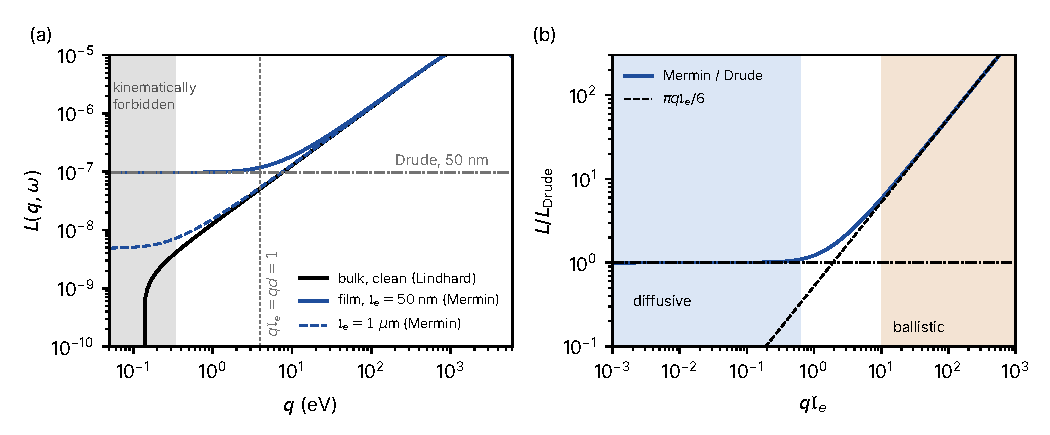
\includegraphics[width=\linewidth]{figures/ch15/fig15_2.pdf}
  \caption{Normal-state loss function of aluminum in a film and in the bulk. (a) $L(q,\omega)$ at $\omega = \SI{0.90}{meV}$ ($5\Delta_{\mathrm{BCS}}$ with the bulk gap) against the momentum transfer $q$, for a free-electron gas with $k_{\mathrm{F}} = \SI{1.75}{\angstrom^{-1}}$ and $v_{\mathrm{F}} = \num{6.75e-3}$. Curves: clean Lindhard function (black), Mermin function with mean free path $\mathfrak{l}_e = \SI{50}{nm}$ (blue, $\gamma_{\mathrm{rel}} = \SI{26.7}{meV}$) and $\mathfrak{l}_e = \SI{1}{\micro m}$ (blue dashed), and the Drude tail $\omega\gamma_{\mathrm{rel}}/\omega_p^2$ for \SI{50}{nm} (gray). Gray band: $q < \omega/v_{\mathrm{max}}$, out of reach of halo dark matter. Dotted vertical line: $q\mathfrak{l}_e = 1$, which for this film is also $qd_{\mathrm{film}} = 1$. (b) Ratio of the Mermin loss function to the Drude tail, against $q\mathfrak{l}_e$, for $q \ll k_{\mathrm{F}}$ (\cref{eq:15.3-mermin}) and $\omega/\gamma_{\mathrm{rel}} = 0.034$; dashed, the ballistic asymptote $\pi q\mathfrak{l}_e/6$. Shaded: within \SI{10}{\percent} of the diffusive limit (left) and of the ballistic limit (right), that is a ratio to the limit of at most 1.1.}
  \label{fig:15-film}
\end{figure}

\Cref{fig:15-film}a shows the consequence for aluminum. At the smallest momentum transfer that can deposit \SI{0.90}{meV}, $q = \omega/v_{\mathrm{max}} = \SI{0.34}{eV}$, the \SI{50}{nm} film has a loss function 24 times that of the clean crystal. The asymptotic $6/\pi q\mathfrak{l}_e$ is 22; the clean value lies below its own small-$\omega$ form there, since $\omega/qv_{\mathrm{F}} = 0.39$. The enhancement persists up to $q \approx 1/\mathfrak{l}_e = \SI{3.9}{eV}$, which is the largest momentum transfer of dark matter lighter than \SI{0.75}{keV}, and above that the two curves merge. A film with $\mathfrak{l}_e = \SI{1}{\micro m}$ lies between. Collisions in a film thus change the loss function for keV-mass dark matter, whereas at the momentum transfers of MeV-mass dark matter the film electrons are ballistic.

The plasmon width and the relaxation rate are different numbers. A Drude form fitted to the measured aluminum plasmon has $\omega_p = \SI{14.9}{eV}$ and a width of \SI{0.863}{eV}~\cite[Fig.~S1]{hochberg2021determining}, 32 times the relaxation rate of the \SI{50}{nm} film. The plasmon decays into electron--hole pairs by interband transitions and by collisions alike, while the tail at meV energies, by \cref{eq:15.3-limits}, is set by the dc resistivity, which measures momentum relaxation at the Fermi surface only. A tail extrapolated from the plasmon width overstates the loss function of the \SI{50}{nm} film at meV energies by that factor of 32.

The logarithms of the Lindhard function and of the BCS bubbles are taken on the retarded branch \cref{eq:C.8-branch}, which the limit of a vanishing width does not select by itself. The other branch suppresses the computed rate of an aluminum detector at low mass by up to seven orders of magnitude~\cite{hochberg2021determining}. A time-ordered bubble coincides with the retarded one at $T = 0$ only for $\omega > 0$, whereas a Kramers--Kronig integral and a sum rule need $\omega < 0$ as well.

\subsection{The superconducting film}\label{sec:15.3-sc}

On the kinematic edge of $y = \omega/\Delta_{\mathrm{BCS}} = 2.2$ the momentum transfer is $q = 2.2\,\Delta_{\mathrm{BCS}}/v_{\mathrm{max}} = \SI{0.15}{eV}$, whatever $v_{\mathrm{F}}$ is, so an aluminum film with $\mathfrak{l}_e = \SI{30}{nm}$ has $q\mathfrak{l}_e = 0.023$ there. Its electrons are diffusive on the scale of the probe, and the clean response of \cref{sec:15.1} does not apply. The conserving response with Born scattering by nonmagnetic impurities at $T = 0$ replaces it. In Nambu space the impurity potential couples through $\boldsymbol{\eta}$, the Nambu matrix of the density, so the Born self-energy is $\boldsymbol{\eta}\,\GF\,\boldsymbol{\eta}$ averaged over the Fermi surface. The same impurity ladder dresses the density vertex and the two pair vertices; with both, the response stays conserving (\cref{app:E.20}). Its normal state is the Mermin function \cref{eq:4.5-mermin} at the same relaxation rate $\gamma_{\mathrm{rel}} = v_{\mathrm{F}}/\mathfrak{l}_e$. \Cref{tab:15-edge} lists its edge values for \SI{1}{\micro m} and \SI{30}{nm}, divided by $\mathfrak{g}_{\mathrm{I}}$ times that normal state, and we use the same normalization for every number in this subsection.

At $y \ge 3$ the ratio hardly moves: it stays between 1.008 and 1.091 for every mean free path from \SI{100}{\micro m} down to \SI{30}{nm}. At $y \le 2.5$, however, it moves a great deal. At $y = 2.2$ it falls from 0.87 in the clean limit to 0.60 at $\mathfrak{l}_e = \SI{1}{\micro m}$, 0.38 at \SI{300}{nm} and 0.19 at \SI{30}{nm}, and at $y = 2.5$ from 1.00 to 0.57. The clean values hold to \SI{4}{\percent} down to $y = 2.2$ only for $\mathfrak{l}_e \ge \SI{10}{\micro m}$. In a film the suppression near the threshold therefore returns, now through the inductive response of the condensate.

The local limit of short mean free path shows why. When $q\mathfrak{l}_e \ll 1$ and $D_{\mathrm{diff}}q^2 \ll \Delta_{\mathrm{BCS}}$, neither an electron nor a pair resolves the spatial variation of the potential, and the film responds locally. The induced density then follows from the induced current by the continuity equation, longitudinal and transverse responses coincide (\cref{eq:4.4-ET}), and $\varepsilon = 1 + \ii\sigma_{\mathrm{cond}}(\omega)/\omega$ by \cref{eq:4.4-sigma}, in the superconducting state as in the normal one. The conductivity of a dirty superconductor is the Mattis--Bardeen conductivity, derived in \cref{sec:15.4-MB} and \cref{app:D.40}. At $T = 0$ its real part $\sigma_1/\sigma_n$ is the case-II pair-creation integral of \cref{eq:7.2-pairspec}, which is zero below $2\Delta_{\mathrm{BCS}}$ and rises continuously from zero above it. Its imaginary part $\sigma_2$ is the Kramers--Kronig partner of $\sigma_1$, and it contains the weight $(\pi^2/2)\Delta_{\mathrm{BCS}}\sigma_n$ missing from $\sigma_1$ below $2\Delta_{\mathrm{BCS}}$, which the condensate carries at $\omega = 0$. Since $|\varepsilon| \gg 1$, $-1/\varepsilon = \ii\omega/\sigma_{\mathrm{cond}}$, and
\begin{equation}
  L = \frac{\omega\,\sigma_1}{\sigma_1^2 + \sigma_2^2}, \qquad
  \frac{L_{\mathrm{s}}}{L_{\mathrm{n}}} = \frac{\sigma_n\,\sigma_1}{\sigma_1^2 + \sigma_2^2} \qquad (q\mathfrak{l}_e \ll 1,\ D_{\mathrm{diff}}q^2 \ll \Delta_{\mathrm{BCS}}) ,
  \label{eq:15.3-MB}
\end{equation}
with $L_{\mathrm{n}} = \omega/\sigma_n$ the Drude tail of \cref{eq:15.3-limits} and $L_{\mathrm{s}}$ the superconducting loss function. Near the threshold the ratio is small for two reasons. By continuity the density couples through the current, which is odd under time reversal, so the coherence factor is that of case~II, which vanishes at $2\Delta_{\mathrm{BCS}}$, rather than that of case~I with its step of $\pi/2$. And $\sigma_2$ exceeds $\sigma_1$ there, 0.757 against 0.139 times $\sigma_n$ at $y = 2.2$: the supercurrent of the condensate short-circuits the slow potential. Divided by $\mathfrak{g}_{\mathrm{I}}$, the normalization of \cref{tab:15-edge}, \cref{eq:15.3-MB} gives 0.157 at $y = 2.2$, 0.985 at $y = 3$, 1.094 at $y = 5$ and 1.023 at $y = 10$, against 0.187, 1.008, 1.091 and 1.021 in the \SI{30}{nm} column: \cref{eq:15.3-MB} is the end point of the table, and it needs only the measured conductivity of the film. At \SI{30}{nm} and $y = 2.2$ the conserving value still lies \SI{20}{\percent} above the local limit, although $D_{\mathrm{diff}}q^2 = 0.042\,\Delta_{\mathrm{BCS}}$ is already small there; the origin of that excess has not been established.

\subsection{Film thickness}\label{sec:15.3-sheet}

A film thicker than $1/q$ responds as the bulk. Its surfaces spread the momentum along the normal over a range $\sim 1/d_{\mathrm{film}}$, a relative correction of order $1/qd_{\mathrm{film}}$, and they carry surface plasmons near $\omega_p/\sqrt2 \approx \SI{11}{eV}$, far above the energies that dark matter deposits at these momenta. A film thinner than $1/q$ responds as a sheet. The external potential is then uniform across the thickness, and the film responds to its in-plane wavevector $\vect{q}_\parallel$ with the induced density $d_{\mathrm{film}}R(q_\parallel,\omega)\phi$ per area. This sheet of charge produces the potential $e^2/[(\varepsilon_a + \varepsilon_b)q_\parallel]\,\ee^{-q_\parallel|z|}$ per unit density, with $\varepsilon_a$ and $\varepsilon_b$ the dielectric constants of the media on the two sides. The two-dimensional Fourier transform of $e^2/4\pi r$ is $e^2/2q_\parallel$, and the image charges of the two half spaces replace the 2 by $\varepsilon_a + \varepsilon_b$. In the bulk the same density produces $e^2/q^2$. Therefore
\begin{equation}
  \varepsilon_{\mathrm{sh}}(q_\parallel,\omega) - 1 = \frac{q_\parallel d_{\mathrm{film}}}{\varepsilon_a + \varepsilon_b}\,\bigl[\varepsilon(q_\parallel,\omega) - 1\bigr] \qquad (qd_{\mathrm{film}} \ll 1) ,
  \label{eq:15.3-sheet}
\end{equation}
and the screening factor $1/|\varepsilon|^2$ in the structure factor $-2\Imag R/|\varepsilon|^2$ becomes $1/|\varepsilon_{\mathrm{sh}}|^2$, larger by $[(\varepsilon_a + \varepsilon_b)/q_\parallel d_{\mathrm{film}}]^2$ while both dielectric functions are large. For a slab in vacuum this is the leading term in $q_\parallel d_{\mathrm{film}}$ of the exact slab response of Lasenby and Prabhu~\cite[Eq.~(19)]{lasenby2022dark}, whose next term is of relative order $q_\parallel d_{\mathrm{film}}$. A thin metal film screens a long-wavelength potential far less than the bulk, because the field of its induced charge spreads outside it. The factor depends on the direction of $\vect{q}$ through $q_\parallel$, which makes the rate of a thin film directional. For this reason the QROCODILE analysis solves the electrostatic problem of a single \SI{2}{nm} WSi layer in vacuum with a Drude dielectric function; it finds the anisotropy strong at $q \sim \SI{1}{nm^{-1}}$ and already significant at $q \sim \SI{1}{keV}$ for energies above \SI{4}{eV}~\cite[supplement]{baudis2025first}. For the \SI{50}{nm} aluminum film $qd_{\mathrm{film}} = 1$ at $q = \SI{3.9}{eV}$, the same momentum at which $q\mathfrak{l}_e = 1$; for dark matter lighter than \SI{0.75}{keV} the film is a diffusive sheet at every momentum transfer. Stacks of sheets and the full slab need the response of a layered medium, which we do not treat here.

\begin{workedexample}{The Mermin loss function of a \SI{50}{nm} aluminum film}\label{we:15-film}
Take the free-electron gas of aluminum with $k_{\mathrm{F}} = \SI{3.45}{keV}$ and $v_{\mathrm{F}} = \num{6.75e-3}$, for which $k_{\mathrm{TF}} = \SI{4.05}{keV}$ and $\omega_p = \SI{15.78}{eV}$ by \cref{eq:4.4-TF}, and a mean free path $\mathfrak{l}_e = d_{\mathrm{film}} = \SI{50}{nm} = \SI{0.253}{eV^{-1}}$. Then $\gamma_{\mathrm{rel}} = v_{\mathrm{F}}/\mathfrak{l}_e = \SI{26.7}{meV}$ and $D_{\mathrm{diff}} = \SI{5.70e-4}{eV^{-1}}$ (\SI{337}{cm^2.s^{-1}}). Let a dark-matter particle deposit $\omega = 5\Delta_{\mathrm{BCS}} = \SI{0.90}{meV}$ with the bulk gap, at the smallest momentum transfer that allows it, $q = \omega/v_{\mathrm{max}} = \SI{0.340}{eV}$. Then $q\mathfrak{l}_e = 0.086$: the film is diffusive.

\emph{Mermin function.} With $qv_{\mathrm{F}} = \SI{2.29}{meV}$, $\mathfrak{w}_\gamma = 0.392 + 11.62\,\ii$, and \cref{eq:15.3-fL} gives $\mathfrak{f}_{\mathrm{L}} = (2.449 + 0.165\,\ii)\times10^{-3}$, within \SI{0.5}{\percent} of the tail $-1/3\mathfrak{w}_\gamma^2$. \Cref{eq:15.3-mermin} yields $\varepsilon_{\mathrm{Mer}} = (0.407 + 10.35\,\ii)\times10^{6}$, and the diffusion pole \cref{eq:15.3-diff}, with $D_{\mathrm{diff}}q^2 = \SI{0.066}{meV}$, is $(0.755 + 10.33\,\ii)\times10^{6}$: the imaginary parts agree, and the real parts differ at the order $\omega/\gamma_{\mathrm{rel}}$ that the pole drops. The loss function is $L_{\mathrm{Mer}} = \num{9.65e-8}$, \SI{0.2}{\percent} above the Drude tail $\omega\gamma_{\mathrm{rel}}/\omega_p^2 = \num{9.63e-8}$. The same number is $\varepsilon_0\omega\rho_{\mathrm{el}}$ with the residual resistivity \SI{0.80}{\micro\ohm.cm} of \cref{eq:15.3-rho}.

\emph{Comparisons.} The clean Lindhard function at the same point is $\varepsilon_{\mathrm{Lin}} = (1.19 + 0.88\,\ii)\times10^8$, with $L = \num{4.01e-9}$: the film absorbs 24 times more.

\emph{Superconducting film.} The film is dirty ($\mathfrak{l}_e/\xi_{\mathrm{coh}} = 0.021$), and $D_{\mathrm{diff}}q^2 = 0.37\,\Delta_{\mathrm{BCS}}$: \cref{eq:15.3-MB} applies roughly. At $y = 5$ it gives $L_{\mathrm{s}}/L_{\mathrm{n}} = 1.259$ and $L_{\mathrm{s}} = \num{1.21e-7}$. In the normalization of \cref{tab:15-edge} that is 1.094, and clean, intermediate and dirty films lie between 1.057 and 1.094 at this energy, within \SI{4}{\percent}; at $y = 2.2$ the clean value is 5.5 times the local limit.

\emph{Thickness.} Finally $qd_{\mathrm{film}} = 0.086$: the film is a sheet at this momentum, and in vacuum \cref{eq:15.3-sheet} reduces the screening by $q_\parallel d_{\mathrm{film}}/2$ for $\vect{q}$ in the plane, which multiplies the structure factor by $(2/0.086)^2 = 540$ to leading order in $q_\parallel d_{\mathrm{film}}$; the exact slab response of Lasenby and Prabhu gives 588. The bulk loss function computed here is the input to the sheet response, not the final answer.
\end{workedexample}

\subsection{Amorphous tungsten silicide}\label{sec:15.3-wsi}

Amorphous W$_x$Si$_{1-x}$ has no lattice, and its transport is measured, not computed. In \SI{5}{nm} films with $x = 0.75$--0.85 the sheet resistance, the resistance of a square of film, is 326--\SI{417}{\ohm}, a resistivity $\rho_{\mathrm{el}} = R_\square d_{\mathrm{film}}$ of 163--\SI{209}{\micro\ohm.cm}, 205 to 263 times that of the aluminum film of \cref{we:15-film}~\cite[Table~I]{zhang2016characteristics}. The magnetic field that destroys superconductivity rises below $T_c$ at a rate set by how fast the electrons diffuse, and its slope yields the diffusion constant 0.70--\SI{0.75}{cm^2.s^{-1}}. In a diffusive conductor the current is the diffusion current of the electrons that a field pushes off equilibrium, so the conductivity is $\sigma = e^2(2\mathcal{N}_{\mathrm{F}})D_{\mathrm{diff}}$, the Einstein relation. With the measured resistivity and diffusion constant of each film it gives the density of states $2\mathcal{N}_{\mathrm{F}} = $ (2.7--3.3)$\times10^{47}$\,m$^{-3}$\,J$^{-1}$, and at most \num{3.4e47}\,m$^{-3}$\,J$^{-1}$ for any combination of the measured values. The Ginzburg--Landau coherence length, the size of a pair measured near $T_c$, is 7.0--\SI{7.4}{nm}, and $T_c$ is 3.8--\SI{4.1}{K}. The \SI{2}{nm} W$_{0.45}$Si$_{0.55}$ layer of the QROCODILE detector has $T_c = \SI{1.73}{K}$~\cite{baudis2025first}, which gives $\Delta_{\mathrm{BCS}} = 1.764\,T_c = \SI{0.263}{meV}$.

The free-electron gas at $E_{\mathrm{F}} = \SI{7}{eV}$ has $k_{\mathrm{F}} = \SI{2.67}{keV}$, $v_{\mathrm{F}} = \num{5.23e-3}$ and $2\mathcal{N}_{\mathrm{F}} = \SI{1.13e47}{m^{-3}.J^{-1}}$. The density of states from the Einstein relation is 2.4--2.9 times larger: the gas does not describe these electrons, and the mean free path depends on which free-gas number is combined with the data. With the measured $D_{\mathrm{diff}}$ and \cref{eq:15.3-le}, $\mathfrak{l}_e = 3D_{\mathrm{diff}}/v_{\mathrm{F}} = 0.13$--\SI{0.14}{nm} and $k_{\mathrm{F}}\mathfrak{l}_e = 1.8$--1.9. With the measured resistivity and the free-gas $\omega_p = \SI{10.8}{eV}$, $\gamma_{\mathrm{rel}} = \varepsilon_0\omega_p^2\rho_{\mathrm{el}} = 2.5$--\SI{3.3}{eV}, $\mathfrak{l}_e = 0.32$--\SI{0.41}{nm} and $k_{\mathrm{F}}\mathfrak{l}_e = 4.3$--5.5. Either way $k_{\mathrm{F}}\mathfrak{l}_e = 2E_{\mathrm{F}}/\gamma_{\mathrm{rel}}$ is a few: the relaxation rate is comparable with the Fermi energy and the mean free path with the electron wavelength $2\pi/k_{\mathrm{F}} = \SI{0.46}{nm}$.

At the momentum transfers of MeV-mass dark matter, $q = 1$ to \SI{5}{keV}, this leaves no small parameter. There $q/k_{\mathrm{F}} = 0.37$--1.9 and $q\mathfrak{l}_e = 0.7$--3.4 with the shorter mean free path, while \cref{eq:15.3-fL} needs $q \ll k_{\mathrm{F}}$, the limits \cref{eq:15.3-limits} need $q\mathfrak{l}_e$ far from one, and a relaxation time itself needs $k_{\mathrm{F}}\mathfrak{l}_e \gg 1$, so that an electron has a momentum to relax. The Mermin function and its two limits are then all outside the conditions under which they were derived, and no correction factor to any of them can be quoted. At the pair-breaking edge the situation is the opposite. There $q = 2\Delta_{\mathrm{BCS}}/v_{\mathrm{max}} = \SI{0.20}{eV}$ and $q\mathfrak{l}_e \approx 10^{-4}$, and the diffusion pole \cref{eq:15.3-diff} holds for any conductor, since it needs only the continuity equation and Ohm's law with the Einstein relation. The normal-state loss function there is $\varepsilon_0\omega\rho_{\mathrm{el}} = (1.2$--$1.5)\times10^{-5}$ at $\omega = 2\Delta_{\mathrm{BCS}}$, fixed by the measured resistivity.

The superconducting part lies outside mean-field BCS. WSi is deep in the dirty limit, $\mathfrak{l}_e/\xi_{\mathrm{coh}} \approx 0.02$, where Anderson's theorem would keep the clean gap and \cref{eq:15.3-MB} would give the edge. But the theorem rests on disorder being weak: the density of states of the exact states, and the attraction between partners, change at relative order $1/k_{\mathrm{F}}\mathfrak{l}_e$, which is not small here. In addition, slow diffusion enhances the Coulomb repulsion between electrons, the Altshuler--Aronov effect. The enhanced repulsion competes with the pairing attraction and lowers $T_c$, the Finkel'stein mechanism~\cite[Sect.~III.2]{sacepe2020quantum}. BCS theory contains neither, and in strongly disordered films the gap also varies from place to place.

The rate of an amorphous film therefore needs the configurational average of the loss function over the amorphous structures, $\langle\Imag[-(\varepsilon^{-1})_{\vect{0}\vect{0}}]\rangle$, and the distribution of the local gap (\cref{app:E.20}). The average differs from the loss function of the averaged $\varepsilon$ at the order of the variance of $\varepsilon$. Both are open for amorphous WSi at momentum transfers of a keV.
